\section{Introductory Example} 

Inj this section, we present a simple example to give an overview our Verilog to C translation and to illustrate how properties for safety verification written in System Verilog Assertions (SVA) will also be translated also C code for our experiments. We assume the reader is familiar with the basics of Verilog and SVA~\cite{verilog}. \tmcmt{Rajdeep: what are best references?}

Fig.~\ref{fig:example} shows a typical Verilog module with a variety of common constructs: register datatypes, initialization, non-blocking and blocking assignments, an assign statement, and procedural blocks.  The synthesized hardware is the simple circuit shown in the centre.  On the right is the result of our translation of this Verilog RTL code into C.

The details of the translation are explained in Sec.~\ref{sec:v2c}. In summary, however, all the state-holding registers in the Verilog design have been gathered into a C struct. A C function \texttt{top} is then defined that has the same paramaters as the Verilog module is represents. When invoked, this function executes a sequence of state updates that simulate a single clock-cycle of hardware execution, according to the Verilog synthesis semantics. Because this is a sequentialization of the parallel register updates modelled by the Verilog, some shadow variables are introduced that record register values at the start of the clock cycle for subsequent use. Note that the non-synthesizable Verilog initial block is not included here, as this is a testbench component. Note also that placement of the assignment to \texttt{c} at the end of the body of \texttt{top} follows the `read after write' semantics for Verilog combinational logic.

In our experiments, we compare safety verification of SVA properties of Verilog RTL and software analysis tools of the corresponding C code. We therefore translate SVA into equivalent C code. Fig.~\ref{fig:sva} shows a typical collection of SVA properties that could be checked to hold for our example Verilog module with an RTL verification tool. They are all conditional properties over bounded but varying numbers of clock cycles. The corresponding C is shown on the right. After a block of assignments that do the initialization, we have a non-terminating while-loop that models an infinitely-running system. In each iteration, there is a sequence of calls to the function \texttt{top} that, in effect, advances the clock. These are interspersed with checks of the consequents of the SVA implications, in the right clock cycle and under each implication's antecedet. We discuss property translation in more detail in Sec.~\ref{sec:props}.

\begin{figure*}[t]
\begin{center}
\small
\begin{tabular}{@{}lcl@{}} 
\hline\noalign{\vskip0.25ex}
\textbf{Verilog RTL} & \multicolumn{1}{l}{\textbf{Synthesized Hardware}} & \textbf{Software Netlist} \\
\hline
\begin{lstlisting}[mathescape=true,language=Verilog,basicstyle=\scriptsize\ttfamily]
module top(clk, a, c, out); 
input clk , a;
output [1:0] c;
output reg [3:0] out;
reg b,e; reg [1:0] d;
initial begin
  b=0;d=2'b0;
  e=0;out=4'b0;
end
assign c = e ? 1'b0 : d; 
always @(posedge clk) 
begin
 b<=a;
 if(b) e <= b; 
 else  e <= 0; 
 d <= e + 1;
end
always @(posedge clk) 
begin
  out <= d*d;
end  
endmodule
\end{lstlisting}
&
\begin{minipage}{4.3cm}
\centering
\scalebox{.6}{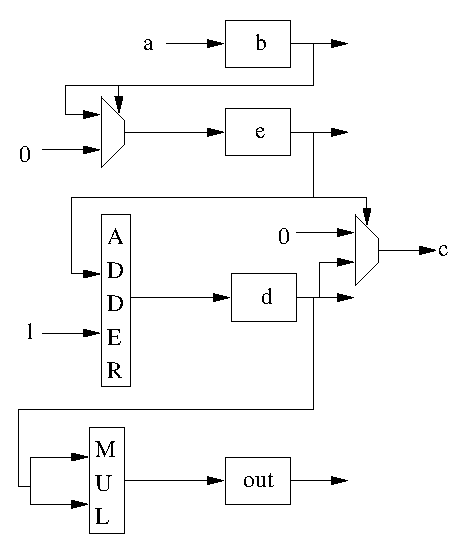
\includegraphics{figures/example/ckt_pspdftex.eps}}
\end{minipage}
&
\begin{lstlisting}[mathescape=true,language=C,basicstyle=\scriptsize\ttfamily]
struct state_elements_top {
  unsigned int b,e;
  unsigned char d,out;
};
struct state_elements_top u1;

void top(unsigned int clk, 
 unsigned int a, 
 unsigned char *c, 
 unsigned char *out) {
 // shadow variables 
 unsigned int b_old = u1.b&0x1;
 unsigned char d_old = u1.d&0x3;
 unsigned int e_old = u1.e&0x1;
  
 u1.b = a;
 if(b_old) 
  u1.e = b_old&0x1;
 else
  u1.e = 0;
 u1.d = (e_old+1)&0x3;
 // update the output 
 u1.out = 
 (d_old&0x3) * (d_old&0x3);
 *out = u1.out&0xF;
 *c = u1.e ? 0 : (u1.d&0x3);
}
\end{lstlisting}\\
\hline
\end{tabular}
\caption{Translation of a Simple Circuit in Verilog HDL to a Software Netlist in C}\label{fig:example}
\end{center}
\end{figure*}

\begin{figure*}[bth]
\small
\begin{center}
\begin{tabular}{@{}ll@{}}
\hline\noalign{\vskip0.25ex}
\textbf{System Verilog Assertions} & \textbf{C Translation} \\
\hline
\begin{lstlisting}[mathescape=true,language=Verilog,basicstyle=\scriptsize\ttfamily]
P0: assert property (d >= e);
P1: assert property ((a == 1) 
    |-> ##1 (b == 1));
P2: assert property ((a == 1) 
    |-> ##2 (e == 1));
P3: assert property ((a == 1) 
    |-> ##3 (d == 2));
P4: assert property ((a == 0) 
    |-> ##4 (out == 1));
P5: assert property ((a == 1) 
    |-> ##4 (out == 4));
\end{lstlisting}
&
\begin{lstlisting}[mathescape=true,language=C,basicstyle=\scriptsize\ttfamily]
_Bool Search_highA(int *highA, unsigned int cycle)
{
 for(int i=0;i<100;i++) { 
   if(highA[i]==cycle) { return 1; }
 }
 return 0;
} 

_Bool Search_lowA(int *lowA, unsigned int cycle)
{
 for(int i=0;i<100;i++) { 
   if(lowA[i]==cycle) { return 1; }
 }
 return 0;
} 

int main() 
{
 unsigned int i=1,j=0,k=0;
 int highA[100], lowA[100];
 // initialize highA and lowA
 for(int i=0;i<100;i++) { 
   highA[i]=999; lowA[i]=999;
 }
 unsigned int clk, a;
 unsigned char c, out;
 // initial block 
 u1.b=0;u1.d=0; u1.e=0;u1.out=0; 
 while(i <= 100) {
  if(a==1) {  
   highA[j]=i; 
   j++;
  } 
  else if(a==0) {
   lowA[k]=i;
   k++;
  }
  top(clk,a,&c,&out);
  i=i+1; 
 
  P0:assert(u1.d>=u1.e);
  // properties with antecedent a==1 
  // property with 1 cycle delay
  if (Search_highA(highA, i-1)) 
   P1:assert(u1.b==1);
  // property with 2 cycle delay
  if (Search_highA(highA, i-2))
   P2:assert(u1.e==1); 
  // property with 3 cycle delay
  if (Search_highA(highA, i-3))
   P3:assert(u1.d==2); 
  // property with 4 cycle delay
  if (Search_highA(highA, i-4))
   P5:assert(u1.out==4); 
  // properties with antecedent a==0
  // property with 4 cycle delay
  if (Search_lowA(lowA, i-4)) 
   P4:assert(u1.out==1);
 }
}
\end{lstlisting}\\
\hline
\end{tabular}
	\caption{Property Specification in SVA and C}
\label{fig:sva}
\end{center}
\end{figure*}

The waveform in Figure~\ref{intro-waveform} captures the input-output behavior of the RTL design. 
%The input-output behavior of the software netlist and the RTL in figure~\ref{intro-fig2} matches 
Using state-of-the-art verifiers, we prove that the result of all assertions 
in Figure~\ref{intro-fig3} are the same in the RTL and the software netlist design. 
%
For example, the properties \texttt{P2:assert(u1.d==1);} and \texttt{P3:assert(c==1);} 
hold only for the first cycle in both RTL and software netlist, but fails in the 
subsequent cycles in both the designs.  All other properties 
hold globally in both the designs, that is, these properties are $k$-inductive 
for the same value of $k$ in the RTL and the software netlist design.
%
\begin{figure} 
\begin{center}
  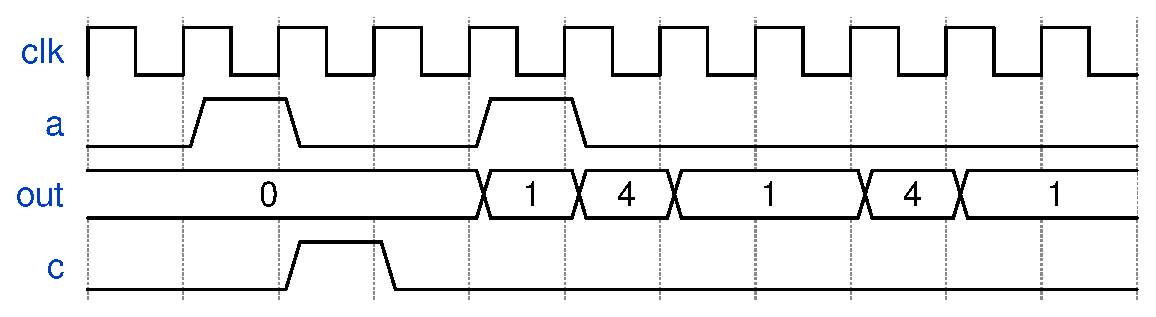
\includegraphics[width=\columnwidth]{figures/example/waveform1.eps}%
	\caption{Waveform showing the Input-Output behavior of RTL in Figure~\ref{intro-fig2}}
\label{intro-waveform}
\end{center}
\end{figure}
%
